\subsection{Input data}
Data set coming from previous steps are used as an input for the calculations in the analysis. These are some of the most relevant features:
\begin{itemize}
    \item unix\_ts\_mne
    \item unix\_ts\_gps
    \item cell\_loc
    \item gps\_loc
    \item class
\end{itemize}

During data gathering we collected 666 mobile network events, however for the majority of them we could not assign a location based on OpenCelliD data set, resulting in only 160 records in the input file. In contrast, using the Telefonica NEXT cell map 640 out of the 666 total were kept.

\begin{figure}[h]
    \begin{minipage}[b]{0.5\textwidth}
        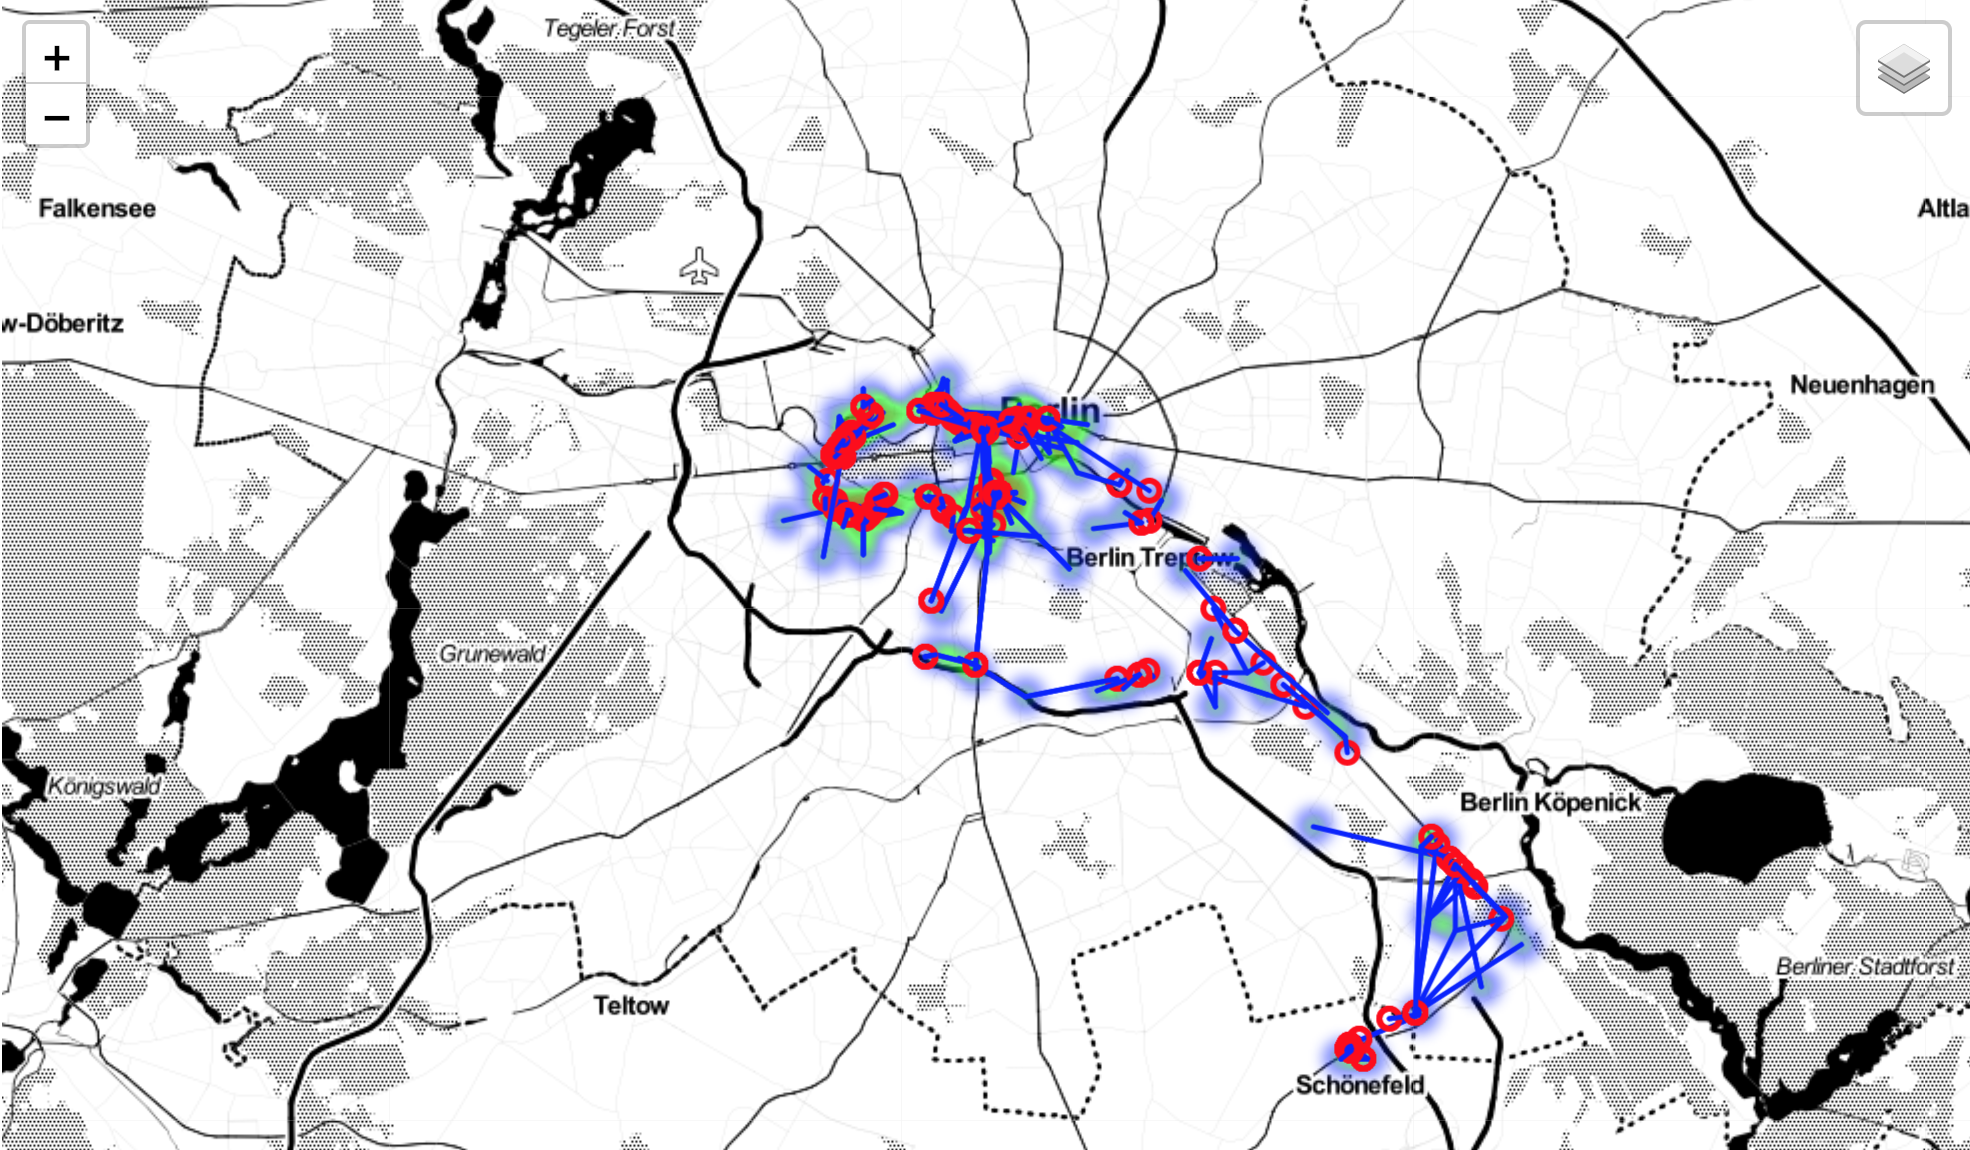
\includegraphics[width=\textwidth]{images/tefnext_traj.png}
        \caption{GPS and CDR trajectories positioned with Telefonica cell map}
        \label{fig:tefnext_avg_threshold}
    
        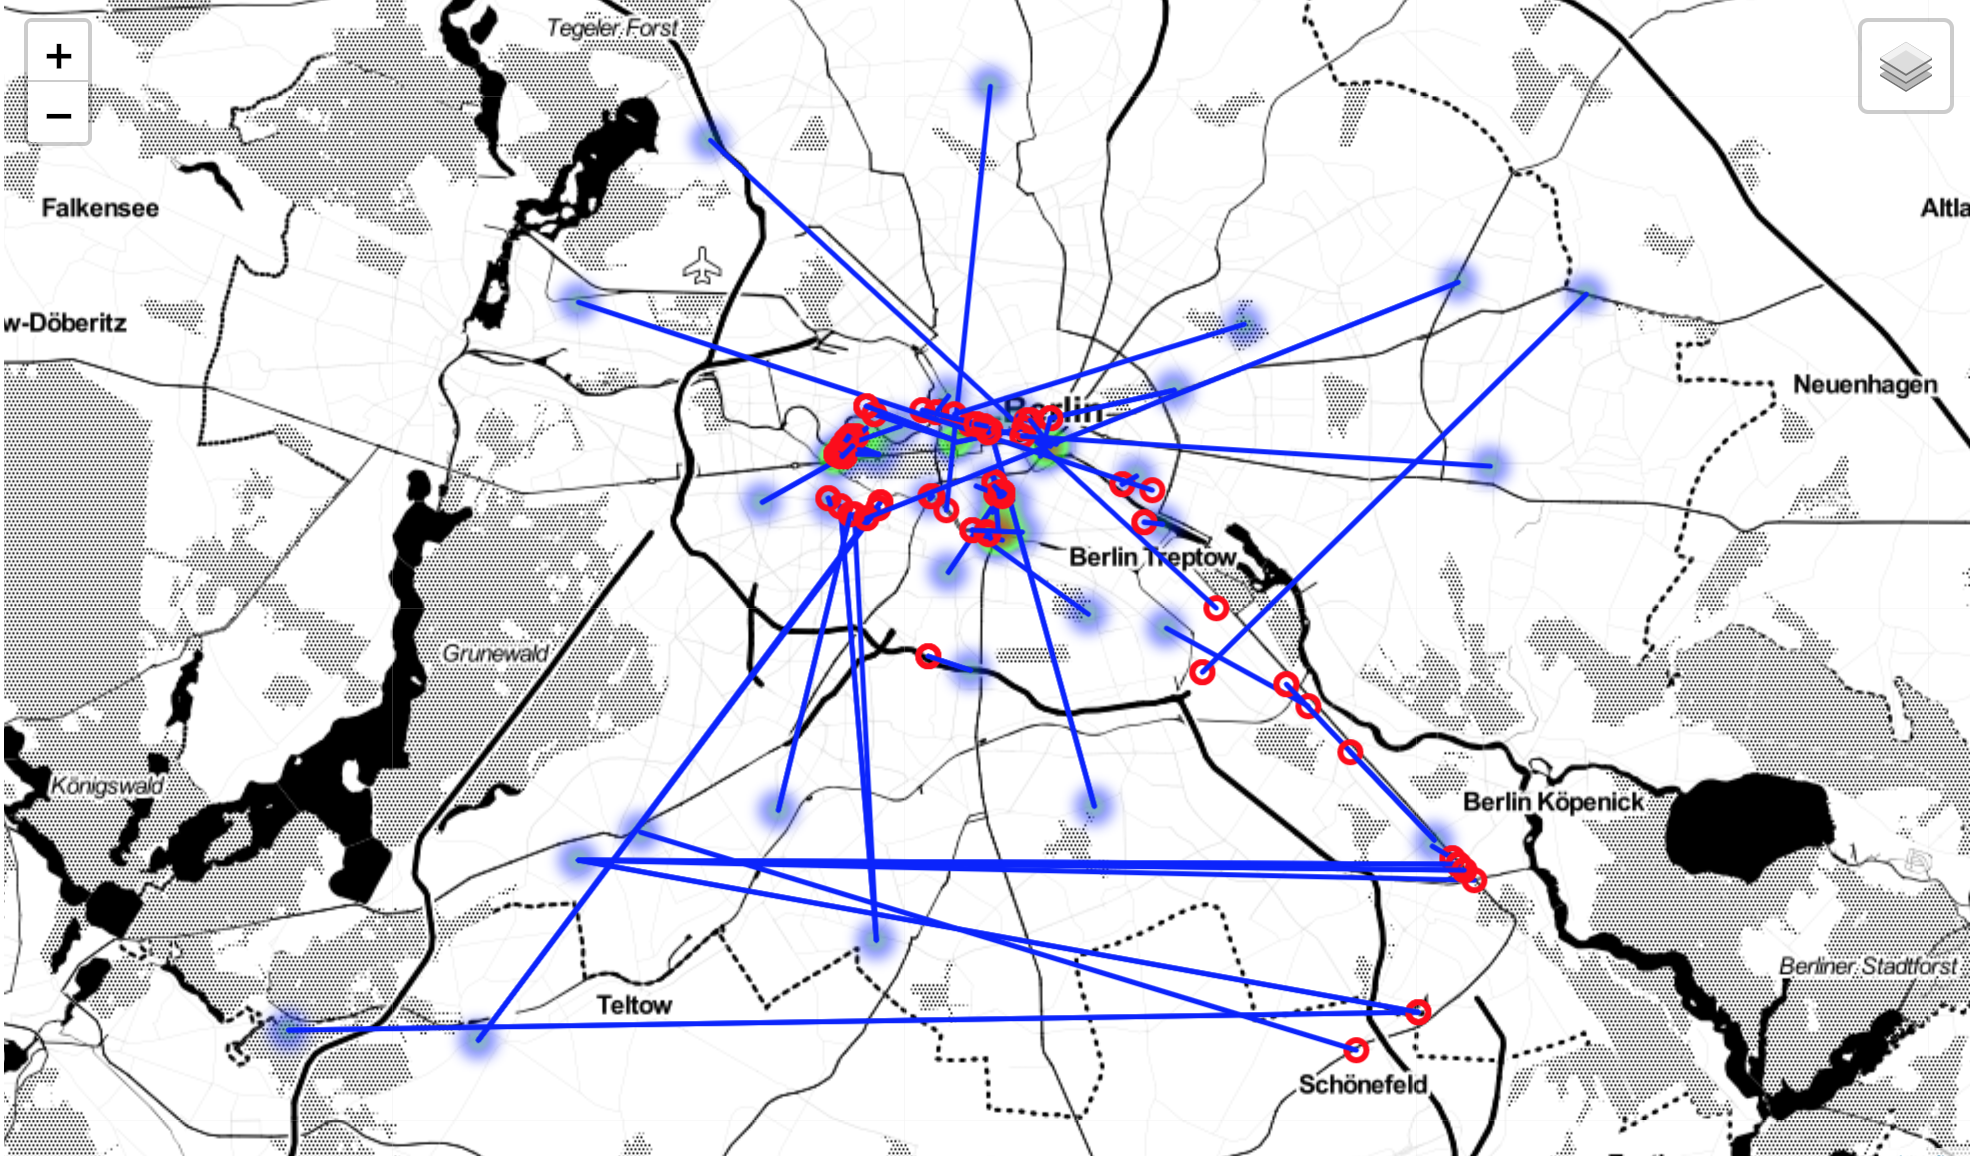
\includegraphics[width=\textwidth]{images/opencellid_traj.png}
        \caption{GPS and CDR trajectories positioned with OpenCelliD cell map}
        \label{fig:opencellid_avg_threshold}
    \end{minipage}\qquad
\end{figure}


\subsection{Steps}
The analysis phase is executed with a following steps:
\begin{enumerate}
    \item Import Parquet data to pySpark DataFrame
    \item Generated and display histograms on pairwise distances
    \item Calculate descriptive statistics on pairwise distances:
        \begin{itemize}
            \item min
            \item max
            \item sum
            \item mean
            \item standard deviation
        \end{itemize}
    \item Calculate Euclidean distance measure on trajectories
    \item Visualize on map
\end{enumerate}

\subsection{Results}

Comparing the trajectories visualized on the map of Berlin on Figure \ref{fig:tefnext_avg_threshold} and Figure \ref{fig:opencellid_avg_threshold} we can immediately tell that the positioning of CDR data-set is less accurate with OpenCelliD cell map than the with Telefonica cell map. This is in line with our expectations, given the OpenCelliD is an open-source project and can contain false information, whereas the cell map data-set from Telefonica contains more accurate data.

\begin{figure}[h!]
    \centering
    \begin{minipage}[b]{0.5\textwidth}
        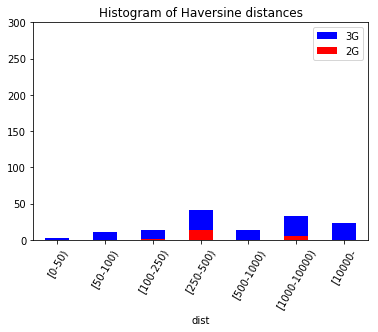
\includegraphics[width=\textwidth]{images/hist_opencell.png}
        \caption{Histogram of distances using OpenCelliD cell map}
        \label{fig:hist_opencell}
    
        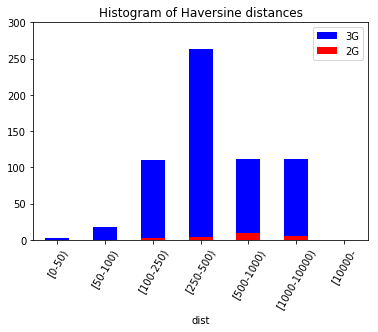
\includegraphics[width=\textwidth]{images/hist_tefnext.png}
        \caption{Histogram of distances using Telefonica cell map}
        \label{fig:hist_tefnext}
    \end{minipage}\qquad
\end{figure}

Looking at the histograms of the pairwise Haversine distances between GPS location points and CDR location point on Figure \ref{fig:hist_tefnext} and Figure \ref{fig:hist_opencell}, we can say that the majority of the distances fall into the 250-500 meters range using both cell maps. 

Overall 62.6\% of the CDR events are positioned with less than 500 meters error. This result can change depending on individual customer's mobile usage habits, network characteristics, cell map data source and the customer's geographical position.

In the OpenCelliD case, there are many observations with larger than 1 km distance and a few larger than 10 kilometers. This explains the 6 kilometers standard deviation shown in Table \ref{tab:dist_stats}, which is quite significant compared to the 700 meters in the Telefonica case. For the latter the maximum distance is 4 kilometers, whereas for OpenCelliD it can go as high as 26 kilometers. This can be due to the fact that OpenCelliD is an open-source project therefore the quality of the observations vary.

The Euclidean distance given the OpenCelliD cell map is significantly larger than of the Telefonica cell map also supporting the argument that the OpenCelliD cell map is not robust enough in Berlin region.

\begin{table}[h]
    \centering
    \begin{tabular}{|l|c|c|}
    	\hline
        Cell map & \textbf{ OpenCelliD} & \textbf{Telefonica} \\
        \hline 
        count & 160 & 640 \\
        \hline
        Euclidean dist & 90635.99 & 25449.76 \\
        \hline
        min(dist) & 44.41 & 22.43 \\
        \hline
        max(dist & 26282.53 & 4020.91 \\
        \hline
        avg(dist) & 3572.21 & 681.89 \\
        \hline
        stddev(dist) & 6230.97 & 740.20 \\
        \hline
    \end{tabular}
    \caption{Descriptive statistics of Haversine distances (in meters)}
    \label{tab:dist_stats}
\end{table}

Most of the CDR events are passive, meaning that most of the events are initiated by the network not the user. We would expect to see significant difference in the average of the distance between active and passive events, however it is not what we found. Due to the fact that the Euclidean distance penalizes the larger values, the difference between the Euclidean distance of active and passive events is much more significant.

The majority of the events occurred on the 3G network and on average these are closer to the actual GPS points than the events on the 2G network in case of Telefonica cell map, but have larger error on average in case of OpenCelliD.

When the user is located between several cell towers, the connection can be passed from one tower to another depending on network traffic fluctuations and other factors. This phenomenon is often referred to as cell tower ping-pong handover. It can however be used for improving positioning and identifying points-of-interest (POIs). As seen in Figure \ref{fig:ping-pong}, the user stays relatively still, but the assigned cell towers change. Without knowing the actual GPS position we can approximate the location of the customer using the ping-pong handover schema.

\begin{figure}[h]
    \centering
    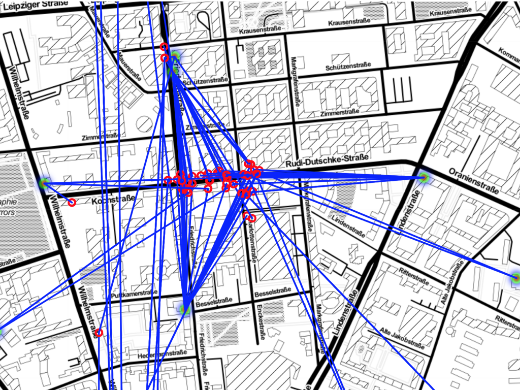
\includegraphics[width=0.5\textwidth]{images/ping-pong.png}
    \caption{Cell ping-pong handover problem}
    \label{fig:ping-pong}
\end{figure}

This method can be further improved if we take into account the angle of the antennas on the cell towers. If we know which antenna is getting the signal, we can guess the direction of the transmitting cell phone and the signal strength can give an approximation of how far away it is. This method is called cell tower triangulation and can be quite accurate in rural regions with more cell towers. However the information about the angles of the antennas and the signal strength can be outdated or even missing therefore it is not always applicable. In this analysis we did not obtain robust data about the positions of the antennas and the signal strength for each CDR event.

Positioning could be improved by reconstructing trajectories considering the road network of Berlin and the potential speed of the movement instead of simply assigning the the cell location from the cell map data. 

%Another improvement is dividing the space into polygonal regions using the Voronoi method can help to delimit the area of influence of each cell tower or antenna. The partitioning is conducted in a way that all points within a given Voronoi cell are closer to its corresponding tower than to any other tower in the surrounding area. This helps to select the cell towers that might reflect the position of the customer with less error on average. \cite{voronoi}

We identified three major external factors defining the accuracy of the positioning:
\begin{itemize}
    \item individual mobile usage habits affecting the sparsity of CDR data,
    \item geographical location, as rural and urban areas has different cell size and therefore location defines the accuracy of cell tower localization and
    \item cellular network characteristics that define the overall data quality and the available attributes in the CDR data-set.
\end{itemize}
